\section{相关技术简介}

\subsection{GNSS(全球卫星导航系统)概述}
全球卫星导航系统(Global Navigation Satellite System,下称GNSS),一般是指通过覆盖全球的导航卫星系统为地面或近地面用户提供全天候的三维空间坐标以及时间信息的无线定位系统。使用GNSS进行定位的用户可以通过具有GNSS信号接收器接收来自当前区域卫星的定位信号,并通过一系列的解码与计算得到较为准确的空间信息与时间信息,从而实现定位、导航、授时(PNT)的功能。

世界上第一个全球卫星导航系统是美国的GPS系统。该系统在设计之初一共由24颗卫星组成,其中21颗为工作卫星,3颗为备用卫星。而截至到目前,GPS系统的卫星数目已经达到了31颗。而在我国,第一颗北斗卫星在2007年4月14日发射,被在往后的若干年里不断完善北斗导航系统。截至2020年,北斗系统已经实现向全球提供服务的目标,与美国GPS、俄罗斯GLONASS、欧盟GALILEO并列成为四大全球定位系统。除了上述的全球性定位系统外,还包括区域系统和增强系统。其中区域系统有日本的QZSS和印度的IRNSS;增强系统则包括美国的WASS、日本的MSAS以及欧盟的EGNOS等。

GNSS的定位原理可以认为是求解一组方程。对于用户所处空间位置$(x_u, y_u, z_u)$,由于导航卫星所处的精确位置是可知的,同时卫星与用户之间的距离也可通过光速与时间差得到,因此可以列出方程(\ref{eq:not_expand_equation})。
\begin{equation}
    \rho_i=\|\textbf{s}_i-\textbf{u}\|
    \label{eq:not_expand_equation}
\end{equation}
其中,$\rho_i$则表示用户距离第$i$颗卫星的距离,$\textbf{S}_i$表示第$i$颗卫星的空间位置,$\textbf{U}$表示用户的空间位置。上述方程可展开为(\ref{eq:1})

\begin{equation}
    \begin{cases}
        \rho_1=\sqrt{(x_1-x_u)^2+(y_1-y_u)^2+(z_1-z_u)^2}\\
        \rho_2=\sqrt{(x_2-x_u)^2+(y_2-y_u)^2+(z_2-z_u)^2}\\
        \rho_3=\sqrt{(x_3-x_u)^2+(y_3-y_u)^2+(z_3-z_u)^2}\\
    \end{cases}
    \label{eq:1}
\end{equation}

其中,$x_i$,$y_i$,$z_i$表示当前用于定位用户位置的第$i$颗卫星的空间位置。求解上述方程组,即可求得用户位置坐标$(x_u,y_u,z_u)$。然而,在实际应用中,除了上述的三个未知数以外,往往还需要第四个未知数$t_u$作为修正项。原因在于,在计算用户位置与卫星间距离时,需要使用导航卫星中的原子钟与地面用户接收器的时钟作差得到钟差,但接收器的时钟精度要比原子钟精度低。这就导致最终得到的钟差会有一定的误差,因此需要加入修正项。此时的方程如(\ref{eq:not_expand_equation_with_bias})所示。
\begin{equation}
    \rho_i=\|\textbf{s}_i-\textbf{u}\|+ct_u
    \label{eq:not_expand_equation_with_bias}
\end{equation}
上式可展开为
\begin{equation}
    \begin{cases}
        \rho_1=\sqrt{(x_1-x_u)^2+(y_1-y_u)^2+(z_1-z_u)^2}+ct_u\\
        \rho_2=\sqrt{(x_2-x_u)^2+(y_2-y_u)^2+(z_2-z_u)^2}+ct_u\\
        \rho_3=\sqrt{(x_3-x_u)^2+(y_3-y_u)^2+(z_3-z_u)^2}+ct_u\\
        \rho_4=\sqrt{(x_4-x_u)^2+(y_4-y_u)^2+(z_4-z_u)^2}+ct_u\\
    \end{cases}
    \label{eq:2}
\end{equation}
其中,$c$表示光速。
\subsection{GNSS位置欺骗攻击及检测方法概述}
目前,GNSS位置欺骗攻击还没有精确的定义。一般而言,“欺骗”是指某人或某程序利用数据篡改、数据伪造等手段成功伪装成另一个人或另一个程序,其目的往往是获取情报或影响被攻击者的正常运作。具体到GNSS位置欺骗攻击方面,攻击者会通过伪造错误定位信号或转发真实卫星信号等手段进行攻击。遭受欺骗攻击的GNSS接收器则会计算出一个错误的位置或错误的时间,从而导致依赖于GNSS定位的其他部件工作受阻或出错,甚至是无法工作。下面将对常见的GNSS位置欺骗攻击手段及检测方法进行简要介绍。
\subsubsection{欺骗方法概述}
\paragraph{基于信号模拟器的自主产生式攻击}

该攻击方式的主要思想是通过一个GNSS信号模拟器发送虚假GNSS定位信号来实现欺骗目的。目前,诸如Spirent公司的GSS8000等GNSS信号模拟器可以模拟出各种真实环境中的卫星定位信号。通过向接收机发送生成的定位信号的方法,可以实现一定程度上的位置欺骗攻击。但这种方法的缺点也很明显。由于GNSS信号模拟器所产生的信号是完全自主产生的,并没有与实际卫星进行信号同步,所以很容易导致接收机出现失锁或重捕的问题,从而导致欺骗被检测。另外,GNSS模拟器庞大的体积以及高昂的价格也是该欺骗方法的主要缺点之一\cite{庞晶2016GNSS}。
\paragraph{基于接收机的接受产生式攻击}

该攻击方式所使用的干扰源主要由两部分组成,即接收机与信号模拟器。接受产生式攻击的基本工作原理与自主产生式攻击类似,都需要使用一个信号模拟器进行信号模拟生产。两者最大的不同在于,前者在产生虚假定位信号时所使用的参数由操作者或机器自身自主设置;而后者则是根据接收机接收到的真是卫星信号的估计结果,通过算法计算得到。与自主产生式攻击相比,接收产生式攻击所产生的信号与真实信号接近,其隐蔽性要更强。而其缺点在于,由于在使用真实卫星信号计算模拟参数时需要精确测定目标接收机与欺骗干扰源之间的三维位置关系,实现难度较大。尤其是当欺骗目标处于运动状态的时候,需要实时测定两者位置关系。也正因如此,这种欺骗手段一般只用于静止状态或低速运动状态下的目标\cite{庞晶2016GNSS}。
\paragraph{基于信号转发器的转发式攻击}
\label{par:zhuanfa}

我国在GNSS欺骗方面的研究主要集中在转发式攻击。该攻击手段所采用的思路与上述两种欺骗方法截然不同。该方法不再生成虚假信号,而是直接使用真实的卫星导航信号,通过使用转发器发射到目标区域,从而使目标接收到另一个空间位置的GNSS定位信号。与产生式攻击方法相比,该方法最大的优点在于不需要了解信号的内部细节(如GNSS信号格式、加密方式等),从而避免了大量技术细节与限制,并因此扩大了适用范围。而该方法的最大缺点在于,由于在信号转发时需要对原始信号放大,这会导致信号中的噪声被一起放大,从而导致转发信号与接收机接收到的真实定位信号在噪声水平上有较大的差别,容易被检测到\cite{庞晶2016GNSS}。
\subsubsection{检测方法概述}
\label{sec:jiance}
\paragraph{基于空间信息处理的检测方法}

该检测方法的主要思想是通过判别导航信号的空间信息来实现欺骗检测。具体来说,GNSS在定位时会从不同方向的不同卫星向用户发送定位信号;而欺骗源往往是从同一方向发射多个信号。通过处理接收到的信号,解算出信号的大致空间特征,就可以识别出当前收到的信号是否为欺骗信号。由于卫星的空间信息几乎是不可能被模仿的,因此这种检测方法是目前最为有效的GNSS欺骗检测方法之一\cite{周彦2022GNSS欺骗检测}。
\paragraph{基于信号到达时间的检测方法}

该检测方法的主要思想是通过判断欺骗信号与真实信号在到达时间上的差异来实现欺骗检测,主要用于转发式攻击。从\ref{par:zhuanfa}中可以看出,当使用欺骗设备对真实信号进行接收并转发后,目标接收机所接收到的信号必然会与真实信号在时间上有一定的延迟。根据这一特征,便可以判断当前是否收到了欺骗攻击。与转发式欺骗攻击方法一样,这种检测方法也是更适用于固定位置的接收机,在动态场景下的适用性有待提高\cite{周彦2022GNSS欺骗检测}。

\paragraph{基于机器学习的检测方法}
机器学习的方法也被应用到GNSS欺骗攻击检测中。举例而言,Semanjski S等人\cite{semanjski2020gnss}将欺骗检测问题转化为分类问题,并使用SVM的方法来区分真实信号与欺骗信号,从而实现检测目的。L.Junzhi等\cite{Junzhi2019gan}探讨了使用生成对抗网络(GAN)来进行GNSS欺骗检测的可行性;Dasgupta等人\cite{dasgupta2021reinforcement}将强化学习(Reinforcement Learning)的方法应用到GNSS的欺骗攻击检测中,通过使用来自自动驾驶汽车的GNSS定位信息、加速度、速度以及方向盘转向角,构建出一个可实现实时(turn-by-turn)欺骗检测的强化学习模型。


\subsection{LSTM概述}
\label{sec:LSTM_gaishu}
长短期记忆(LSTM)网络是深度学习领域处理序列问题的经典模型。该模型以传统的递归神经网络(RNN)为基础,通过增加细胞状态并引入门控电路(即输入门,输出门和遗忘门),有效解决了传统RNN在处理长序列问题时的依赖问题。LSTM网络常被应用于序列问题,如机器翻译、文本生成、语音识别等。在本文中,由于汽车行驶的轨迹可以认为是连续序列,且轨迹点之间是有一定的关系与约束的,因此可以将LSTM网络应用到智能网联汽车的GNSS位置欺骗检测中。图\ref{fig:LSTM_arch}为LSTM网络结构。

\begin{figure}[htbp]
    \begin{center}
        \includegraphics[width=0.8\textwidth]{../graphics/LSTM_basic_arch.eps}
        \caption{LSTM网络结构图}
        \label{fig:LSTM_arch}
    \end{center}
\end{figure}

在LSTM网络中,遗忘门的主要作用是控制当前细胞中信息的权重,并依次决定是否要舍弃信息。其计算公式如下:
\begin{equation}
    f_i^{(t)}=\sigma\bigg(b_i^f+\sum_jU_{i,j}^fx_j^(t)+\sum_jW_{i,j}^fh_j^{(t-1)}\bigg)
    \label{eq:3}
\end{equation}
其中,$\textbf{x}^{(t)}$是当前输入向量,$\textbf{h}^t$是当前隐藏层向量,其中包含所有LSTM细胞的输出。$\textbf{b}^f$、$\textbf{U}^f$、$\textbf{W}^f$分别表示偏置、输入权重和循环权重。$\sigma$表示sigmoid单元,作用是将权重设置为0到1之间的值。

输入门的作用主要是确定当前哪些细胞内的位置需要更新,并计算更新后的值。其计算公式如下所示:
\begin{equation}
    g_i^{(t)}=\sigma\bigg(b_i^g+\sum_jU_{i,j}^gx_j^{(t)}+\sum_jW_{i,j}^gh_j^{(t-1)}\bigg)
    \label{eq:4}
\end{equation}
其中,$\textbf{x}^{(t)}$,$\textbf{h}^t$分别表示当前输入向量与当前隐藏层向量;$\textbf{b}^f$、$\textbf{U}^f$、$\textbf{W}^f$分别表示偏置、输入权重和循环权重。在完成了输入门与遗忘门的计算后,LSTM细胞内部参数会以下方式更新:
\begin{equation}
    s_i^{(t)}=f_i^{(t)}s_i^{(t-1)}+g_i^{(t)}\sigma\bigg(b_i+\sum_jU_{i,j}x_j^{(t)}+\sum_jW_{i,j}h_j^{(t-1)}\bigg)
    \label{eq:5}
\end{equation}
其中,$\textbf{b}$、$\textbf{U}$、$\textbf{W}$分别表示LSTM细胞内的偏置、输入权重和循环权重。

最后,LSTM会计算出最终隐藏层的输出。公式\ref{eq:6}计算出需要输出的细胞状态数值,公式\ref{eq:7}通过$\tanh$函数将细胞状态处理为一个范围在$(-1,1)$内的数值。最后,$q_i^{(t)}$与$h_i^{(t)}$相乘得到当前时刻隐藏层输出。
\begin{equation}
    q_i^{(t)}=\sigma\bigg(b_i^o+\sum_jU^o_{i,j}x_j^{(t)}+\sum_jW_{i,j}^oh_j^{(t-1)}\bigg)
    \label{eq:6}
\end{equation}

\begin{equation}
    h_i^{(t)}=\tanh(s_i^{(t)})q_i^{(t)}
    \label{eq:7}
\end{equation}
其中,$\textbf{b}^o$、$\textbf{U}^o$、$\textbf{W}^o$分别表示偏置、输入权重和输出权重。

\subsection{汽车功能安全概述}
汽车功能安全,一般是指在不存在电子或电气工程系统异常情况下所出现的不合理的危险\cite{刘法旺2021自动驾驶系统功能安全与预期功能安全研究}。与传统汽车相比,智能网联汽车的系统结构更复杂,大量应用了人工智能、协同计算等技术,这使得智能网联汽车的功能安全问题更为突出。目前学界对于功能安全的研究与开发一般遵循ISO 26262标准。该标准由ISO于2011年发布,其中主要包含了以下几点\cite{iso_2018}:
\begin{enumerate}
    \item 如何量化产品的安全等级;
    \item 如何根据不同安全等级设计对应的安全措施;
    \item 如何规避与控制系统性故障及随机故障;
    \item 如何对功能安全进行管理。
\end{enumerate}
另外,该标准中还提出了一种功能失效的危害分析与风险评估方法(Hazard Analysis \& Risk Assessment,HARA),该方法被广泛应用到智能汽车软件开发行业中。具体而言,HARA方法首先对汽车电子电气系统中可能存在的功能安全风险进行分析,然后在此基础上评估风险的严重度S(Severity)、暴露度E(Exposure)以及可控性C(Controllabilit),最终确定各功能安全风险项的汽车安全完成性等级(Automotive Safetv Integration Level,ASIL)。表\ref{tab:HARA_SEC}展示了严重度、暴露度和可控性三个因子的划分标准;表\ref{tab:ASIL}展示了通过S、E、C三个因子确定ASIL等级的依据。ASIL等级由A——D表示,等级越高表示风险程度越高;QM(Quality Management)则表示质量管理,指只需要按照常规开发流程与质量管理体系进行开发即可,不需要增加额外的设计。
\begin{table}
    \begin{center}
    \begin{tabular}{lll}
        \toprule
        严重度S & 暴露度E & 可控性C \\
        \midrule
        S0 无损害 & E0 不可能 & C0 一般可控制\\
        S1 轻度或中度损害 & E1 非常低的概率& C1 简单可控制\\
        S2 严重损害 & E2 低概率& C2 正常可控制\\
        S3 致命损害 & E3 中等概率& C3 难控制或不能控制\\
        \qquad & E4 高概率 & \qquad\\
        \bottomrule
    \end{tabular}
    \end{center}
    \caption{HARA方法中严重度、暴露度与可控性划分标准}
    \label{tab:HARA_SEC}
\end{table}

% Please add the following required packages to your document preamble:
% \usepackage{multirow}
\begin{table}
    \begin{center}
    \begin{tabular}{lllll}
    \toprule
    \multirow{2}{*}{严重程度} & \multirow{2}{*}{暴露概率} & \multicolumn{3}{l}{可控性} \\ \cline{3-5}
                        &                       & C1     & C2     & C3    \\
    \midrule
    \multirow{4}{*}{S1}   & E1                    & QM     & QM     & QM    \\
                        & E2                    & QM     & QM     & QM    \\
                        & E3                    & QM     & QM     & A     \\
                        & E4                    & QM     & A      & B     \\
    \midrule
    \multirow{4}{*}{S2}   & E1                    & QM     & QM     & QM    \\
                        & E2                    & QM     & QM     & A     \\
                        & E3                    & QM     & A      & B     \\
                        & E4                    & A      & B      & C     \\
    \midrule
    \multirow{4}{*}{S3}   & E1                    & QM     & QM     & A     \\
                        & E2                    & QM     & A      & B     \\
                        & E3                    & A      & B      & C     \\
                        & E4                    & B      & C      & D     \\
    \bottomrule
    \end{tabular}
    \end{center}
    \caption{ASIL划分标准}
    \label{tab:ASIL}
\end{table}

本文将参照ISO 2626标准,依据HARA功能安全分析方法,确定各安全风险项目的风险等级,并提出若干可用于响应GNSS位置欺骗攻击的功能安全应急策略,以实现检测算法与应急策略的联动。

\subsection{国内外研究现状}
\subsubsection{智能网联汽车GNSS位置欺骗攻击检测方面}
\paragraph{国外研究现状}
\label{国外研究现状GNSS_guowai}
如\ref{sec:jiance}所述,GNSS位置欺骗攻击检测所采取的方法一般有\romannum{1})基于空间信息处理的检测方法;\romannum{2})基于信号到达时间的检测方法;以及\romannum{3})基于机器学习的检测方法。然而,这些方法并不一定完全适用于智能网联汽车。具体而言,

\paragraph{国内研究现状}
\label{GNSS_guonei}

\subsubsection{智能网联汽车GNSS功能安全方面}
\subsection{本章小结}
本章主要介绍了对本文所涉及到的技术做简要介绍。首先介绍了GNSS的工作原理、GNSS位置欺骗攻击方法及检测方法;紧接着对LSTM网络的基本原理做了概述;接下来介绍了汽车功能安全的概念,以及相关的ISO 26262标准;最后,本章还就国内外学界就智能智能网联汽车GNSS欺骗检测以及功能安全方面的研究现状做了概述。
